\documentclass[10pt]{article}
\usepackage[T1]{fontenc}
\usepackage{lmodern}
\usepackage[letterpaper,margin=0.82in]{geometry}
\usepackage{amsmath}
\usepackage{graphicx}
\usepackage{microtype}
\usepackage[hidelinks,pdftitle={Vibronic absorption and fluorescence with PySCF ESD},pdfauthor={PySCF ESD project}]{hyperref}

\graphicspath{{../benchmarks/}{docs/benchmarks/}}
\newcommand{\wn}{\ensuremath{\mathrm{cm}^{-1}}}
\newcommand{\doi}[1]{\href{https://doi.org/#1}{DOI~\nolinkurl{#1}}}
\setlength{\emergencystretch}{1em}
\renewcommand{\topfraction}{0.85}
\renewcommand{\textfraction}{0.10}
\renewcommand{\floatpagefraction}{0.75}

\title{Vibronic absorption and fluorescence with PySCF ESD}
\author{PySCF ESD project}
\date{}

\begin{document}
\maketitle

\begin{abstract}
PySCF ESD computes electric-dipole absorption and fluorescence from tracked singlet density-functional excited states or from prepared electronic and vibrational inputs. We examine how the choice of vibrational model affects the vibronic origin, band intensities, and absorption--fluorescence peak separation. In benzene, treating soft modes anharmonically improves the fluorescence envelope relative to the harmonic PBE control. In gas-phase pyridine, an adiabatic Hessian calculation with linear Herzberg--Teller coupling gives an origin 2.17\% below experiment and puts the fluorescence envelope too far to the red. For 9-cyanoanthracene in cyclohexane, analytic curvatures and dipole derivatives improve the ratio of two integrated fluorescence bands at the expense of the absolute band maxima. For one conformer of the quinine dication in a water continuum, the calculated absorption peak lies near the measured value in aqueous acid and the peak Stokes separation is underestimated. A periodic-rotor diagnostic for trifluoronitrosomethane reproduces the peak-to-origin interval despite a large absolute offset and an electronically unstable restricted reference.
\end{abstract}

\section{Introduction}

A vertical excitation energy locates an electronic transition at a single geometry. Its absorption and fluorescence bands also depend on the shapes and relative displacement of the electronic surfaces, vibrational populations, and the variation of the transition dipole. In their path-integral treatment, de Souza, Neese, and Izs\'ak examined the effects of these ingredients on calculated fluorescence spectra and radiative rates.\cite{desouza} Here we use PySCF ESD to examine individual observables from DFT calculations with different vibrational models. The comparisons include benzene from that benchmark, a weak gas-phase transition, two further solution spectra, and a torsional diagnostic. Each comparison identifies the computed energy scale and any translation or broadening used to compare band shapes.

\section{Theory and computational methods}

\subsection{Electronic structure}

The default molecular workflow starts from a single geometry and treats isolated, restricted singlet excitations in the Tamm--Dancoff approximation (TDA) with PBE0/def2-TZVPD at 0 K.\cite{pyscf,tda,pbe0,diffuse} It optimizes the ground and selected excited states using analytic gradients. Signed overlaps of particle--hole amplitudes between successive geometries, evaluated with cross-geometry atomic-orbital overlaps, guide root assignment and phase the transition dipoles. Independent residuals qualify the self-consistent field (SCF) and electronic response. Orbital-stability tests at the endpoints probe rotations within the restricted space and toward an unrestricted determinant.\cite{stability} The latter instability blocks the automatic spectrum for that reference. The optional vertical-gradient (VG) model uses the ground-state Hessian and the excited-state gradient at the ground-state minimum to construct two harmonic wells with equal curvature.

The automatic gas-phase adiabatic Hessian (AH) route obtains excited-state curvature and dipole derivatives from checked local fits to analytic gradients and signed dipoles. Separate calculations with prepared, isolated roots can use analytic density-fitted TDA Hessians and dipole derivatives, including equilibrium linear response in a conductor-like polarizable continuum model (C-PCM).\cite{gpu,cpcm} Pyridine and the solution comparisons below use explicitly prepared inputs. Their protocols differ from the default molecular workflow.

\subsection{Vibrational structure and intensities}

In the AH model the mass-weighted coordinates on the two surfaces are related by $Q_f=JQ_i+K$, where $J$ is the Duschinsky rotation and $K$ the displacement following rigid alignment of the two geometries. Independent curvatures enter the vibronic origin through $E_{00}=E_f^{\min}-E_i^{\min}+Z_f-Z_i$, with $E_s^{\min}$ the electronic energy at the minimum and $Z_s$ the harmonic zero-point energy on surface $s$.\cite{santoro} In the equal-curvature adiabatic-shift Franck--Condon (AS--FC) model, the endpoint displacement is retained and the ground-state curvature is used for both surfaces, so the zero-point correction vanishes.

For vibrational states $\chi_{in}$ and $\chi_{fm}$, the absorption or emission line strength is
\begin{equation}
 S_{mn}=\left\lVert
 \left\langle\chi_{fm}\left|
 \boldsymbol{\mu}_0+\sum_k Q_{i,k}\boldsymbol{\mu}'_k
 \right|\chi_{in}\right\rangle\right\rVert^2 .
 \label{eq:strength}
\end{equation}
The constant dipole $\boldsymbol{\mu}_0$ gives the Franck--Condon (FC) term. The first derivatives $\boldsymbol{\mu}'_k$ give the Herzberg--Teller (HT) term. The two amplitudes interfere before squaring.\cite{baiardi} The sticks carry the initial-state Boltzmann populations. Absorption oscillator strengths scale with $E_\gamma S_{mn}$ and spontaneous emission rates with $E_\gamma^3 S_{mn}$ for positive photon energy $E_\gamma$. Computed emission rates use the vacuum radiative prefactor. Experimental fluorescence traces are used for line-shape comparisons.

The automatic workflow uses a default coverage target of 99.5\% for both initial populations and final dipole strength and screens sampled electronic cuts for anharmonicity. A discrete variable representation (DVR) describes a single anharmonic coordinate.\cite{dvr} A separate finite-temperature calculation can combine a supplied periodic rotor and harmonic spectator modes, including their thermal populations through a characteristic function.

For the plots, fluorescence sampled per wavelength is treated as a wavelength density and projected into a photon-energy density with the corresponding Jacobian. The linewidth scan holds the prior rigid shifts fixed and minimizes the experimental-peak-normalized RMSE over each measured energy window. We preserve the physical absorption scale where available and otherwise normalize spectra to their peaks in that window.

\section{Results and discussion}

\subsection{Benzene in \emph{n}-hexane}

The overlays in Fig.~\ref{fig:benzene} include the experiment and the published ORCA AH curves from Fig.~3 of Ref.~\cite{desouza}. At 298 K the PBE anharmonic model combines a radial $E_{2u}$ potential and a quartic $B_{2g}$ continuation. It reproduces all three main fluorescence bands. At the original common linewidth its fluorescence RMSE is 0.100, compared with 0.160 for harmonic PBE. Narrowing the Gaussian component of the Voigt profiles with the shifts fixed lowers the anharmonic RMSE to 0.063 in absorption and 0.081 in fluorescence. Applying the same adjusted widths to harmonic PBE yields 0.066 and 0.131, respectively. The published ORCA traces give 0.085 and 0.071. An archived mixed PBE/B3LYP5 force-field and dipole diagnostic with limiting front-face collection gives fluorescence RMSE 0.074 and area-normalized total variation 0.072, versus 0.071 and 0.080 for ORCA. Its fluorescence maxima remain 0.018--0.022~eV below experiment.

\begin{figure}[!htbp]
  \centering
  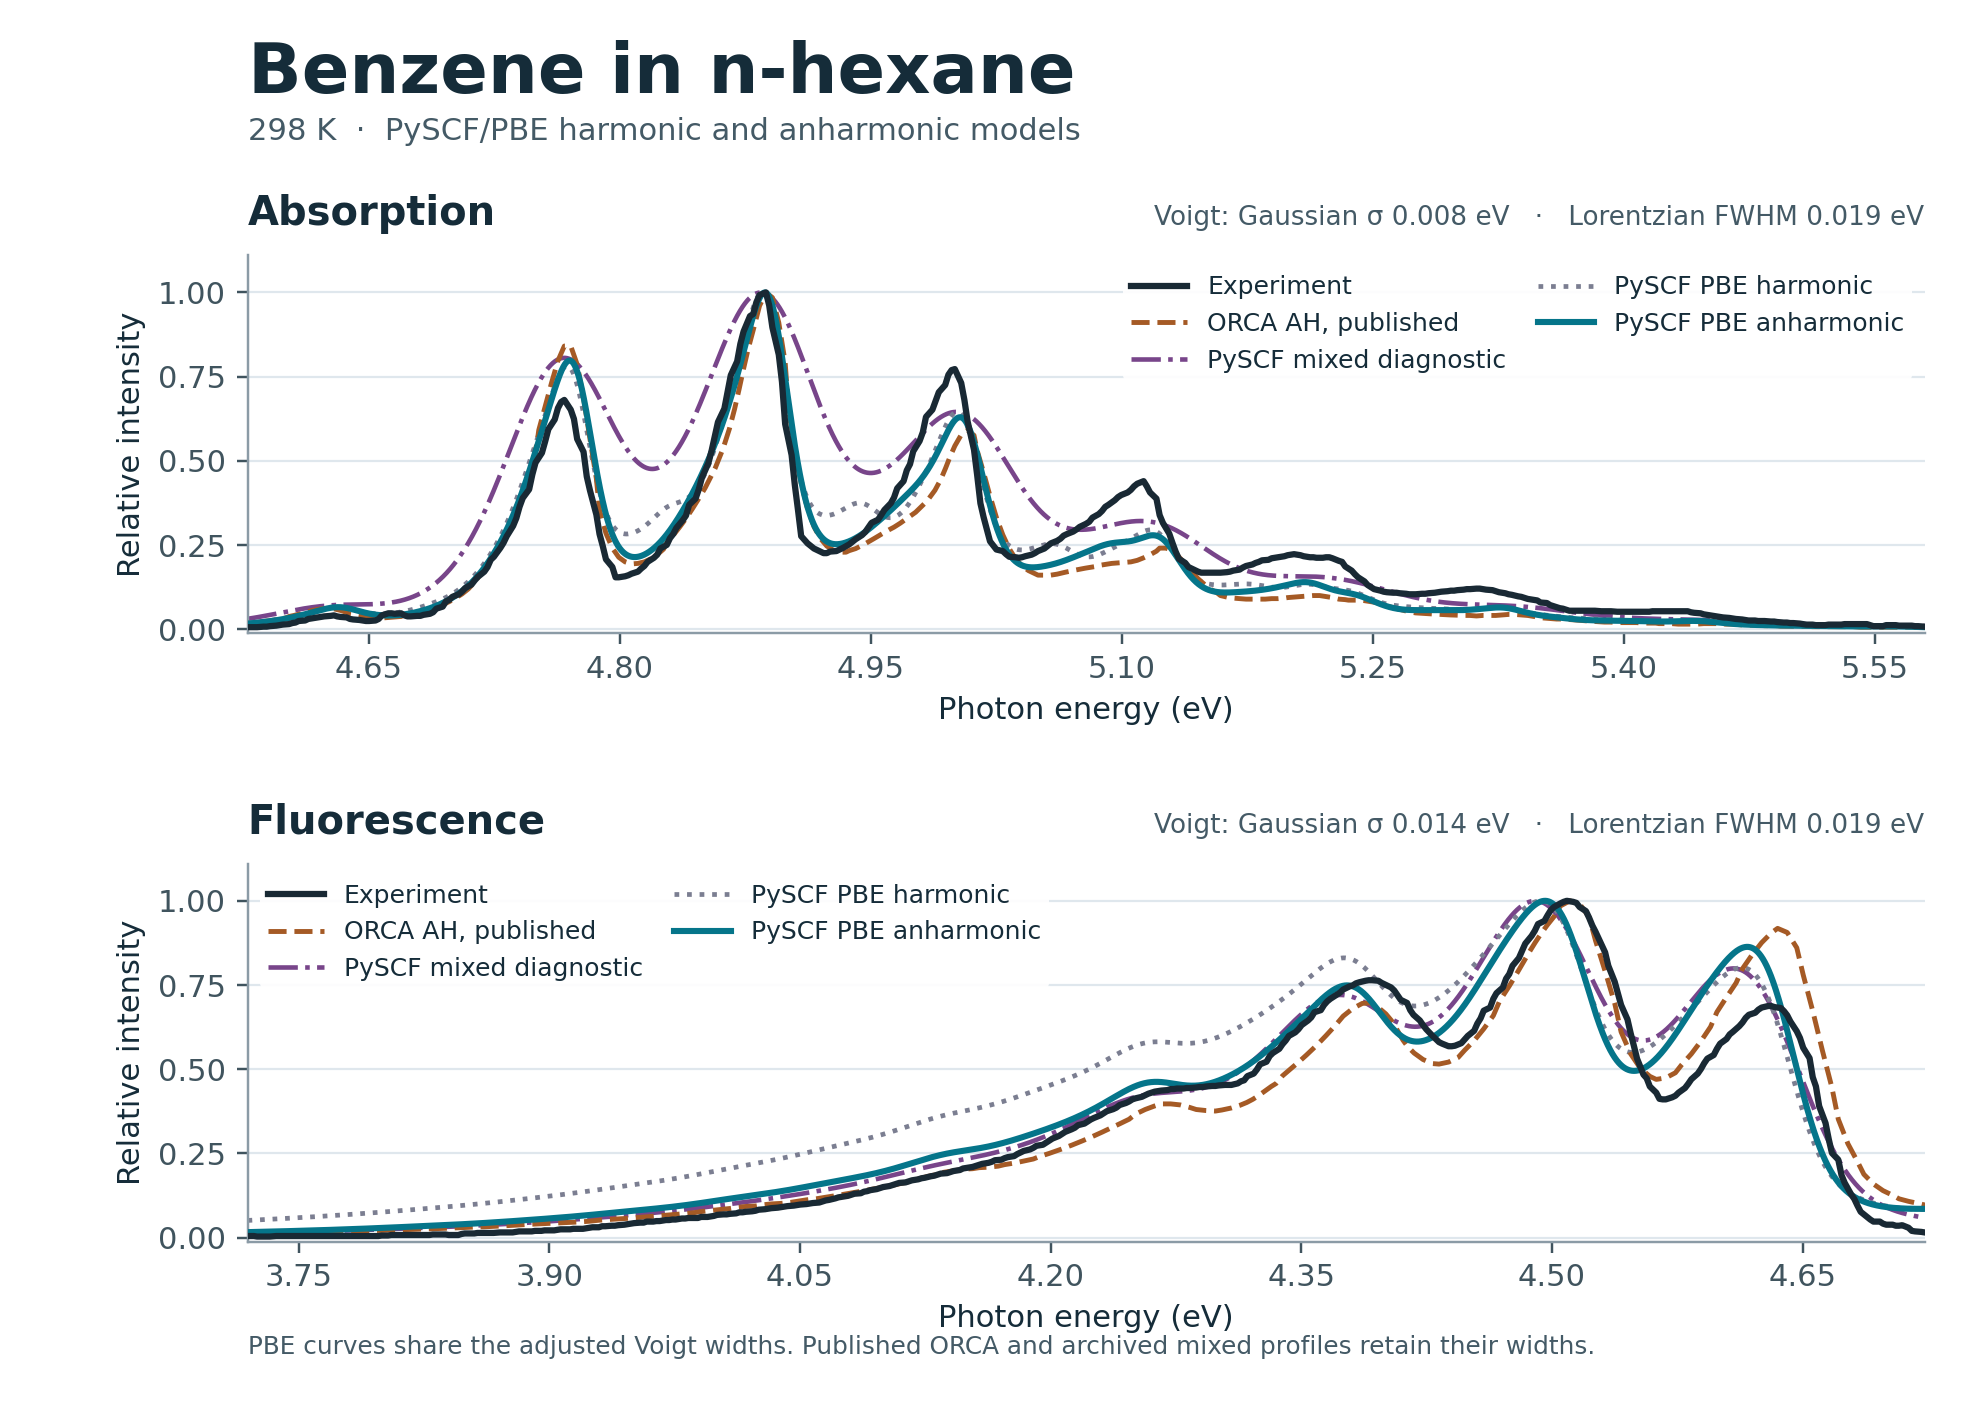
\includegraphics[width=0.88\linewidth]{benzene.png}
  \caption{Absorption and fluorescence of benzene in \emph{n}-hexane. The two PBE models share the adjusted Voigt profiles with Lorentzian FWHM 0.019~eV and Gaussian standard deviations of 0.008~eV for absorption and 0.014~eV for fluorescence. The archived mixed profile uses Gaussian standard deviation 0.025~eV and Lorentzian FWHM 0.019~eV. For both directions, the shifts of the mixed, anharmonic PBE, and harmonic PBE curves are $-0.329$, $-0.241$, and $-0.239$~eV, respectively. The two reference traces are digitized from the published profiles.\cite{desouza}}
  \label{fig:benzene}
\end{figure}

\subsection{Gas-phase pyridine}

At density-fitted PBE0/def2-TZVPD, the tracked $n\pi^*$ singlet has a nonplanar local minimum. We used independent analytic Hessians at the two minima, full Duschinsky rotation, and analytic HT expansions at the initial endpoint of each process. The predicted origin is 34\,012.49~\wn\ versus 34\,767.0~\wn\ in vapor, an underestimate of 754.51~\wn\ (2.17\%).\cite{laane} The zero-point correction is $-1\,681.64$~\wn. The harmonic zero-point energy of the soft out-of-plane mode is 37.11~\wn, above the calculated 0.21~\wn\ barrier to the equivalent well. A local harmonic frequency therefore characterizes the curvature of one well, and the model leaves the motion across the barrier unresolved.

At 298 K the AH+HT integrated absorption oscillator strength is 0.00735, compared with approximately 0.003 for the first measured electronic band.\cite{bolovinos} At 80~\wn\ Gaussian full width at half maximum (FWHM), the calculated absorption accounts for 49\% of the measured area in the 271.0--289.8~nm window. The emission calculation starts in the lowest excited-state vibrational level. The calculated maximum is 29\,062~\wn\ and rises to 29\,816.51~\wn\ with the origin-aligning translation, versus 30\,930~\wn\ in the vapor trace of Yamazaki and Baba as reproduced by Wang and co-workers.\cite{yamazaki,wang} The same translation decreases the peak-normalized emission error from 0.415 to 0.323 in the measured window, while decreasing the calculated absorption area there. The calculated origin gives the stronger agreement of these observables.

\subsection{9-Cyanoanthracene in cyclohexane}

The equal-curvature AS--FC calculation used density-fitted PBE0/def2-SVPD/TDA in equilibrium cyclohexane C-PCM at 293.15 K. Figure~\ref{fig:cyano} compares broadened spectra with the experimental traces of Boens and co-workers.\cite{boens} With the common shift fixed at $+0.025$~eV, widening the Gaussian FWHM from 0.050~eV to 0.108~eV for absorption and 0.112~eV for fluorescence reduces the respective profile RMSE from 0.239 to 0.184 and from 0.231 to 0.170. The strongest calculated absorption remains at the red edge near 3.12~eV, while the measured maximum is near 3.27~eV.

\begin{figure}[!htbp]
  \centering
  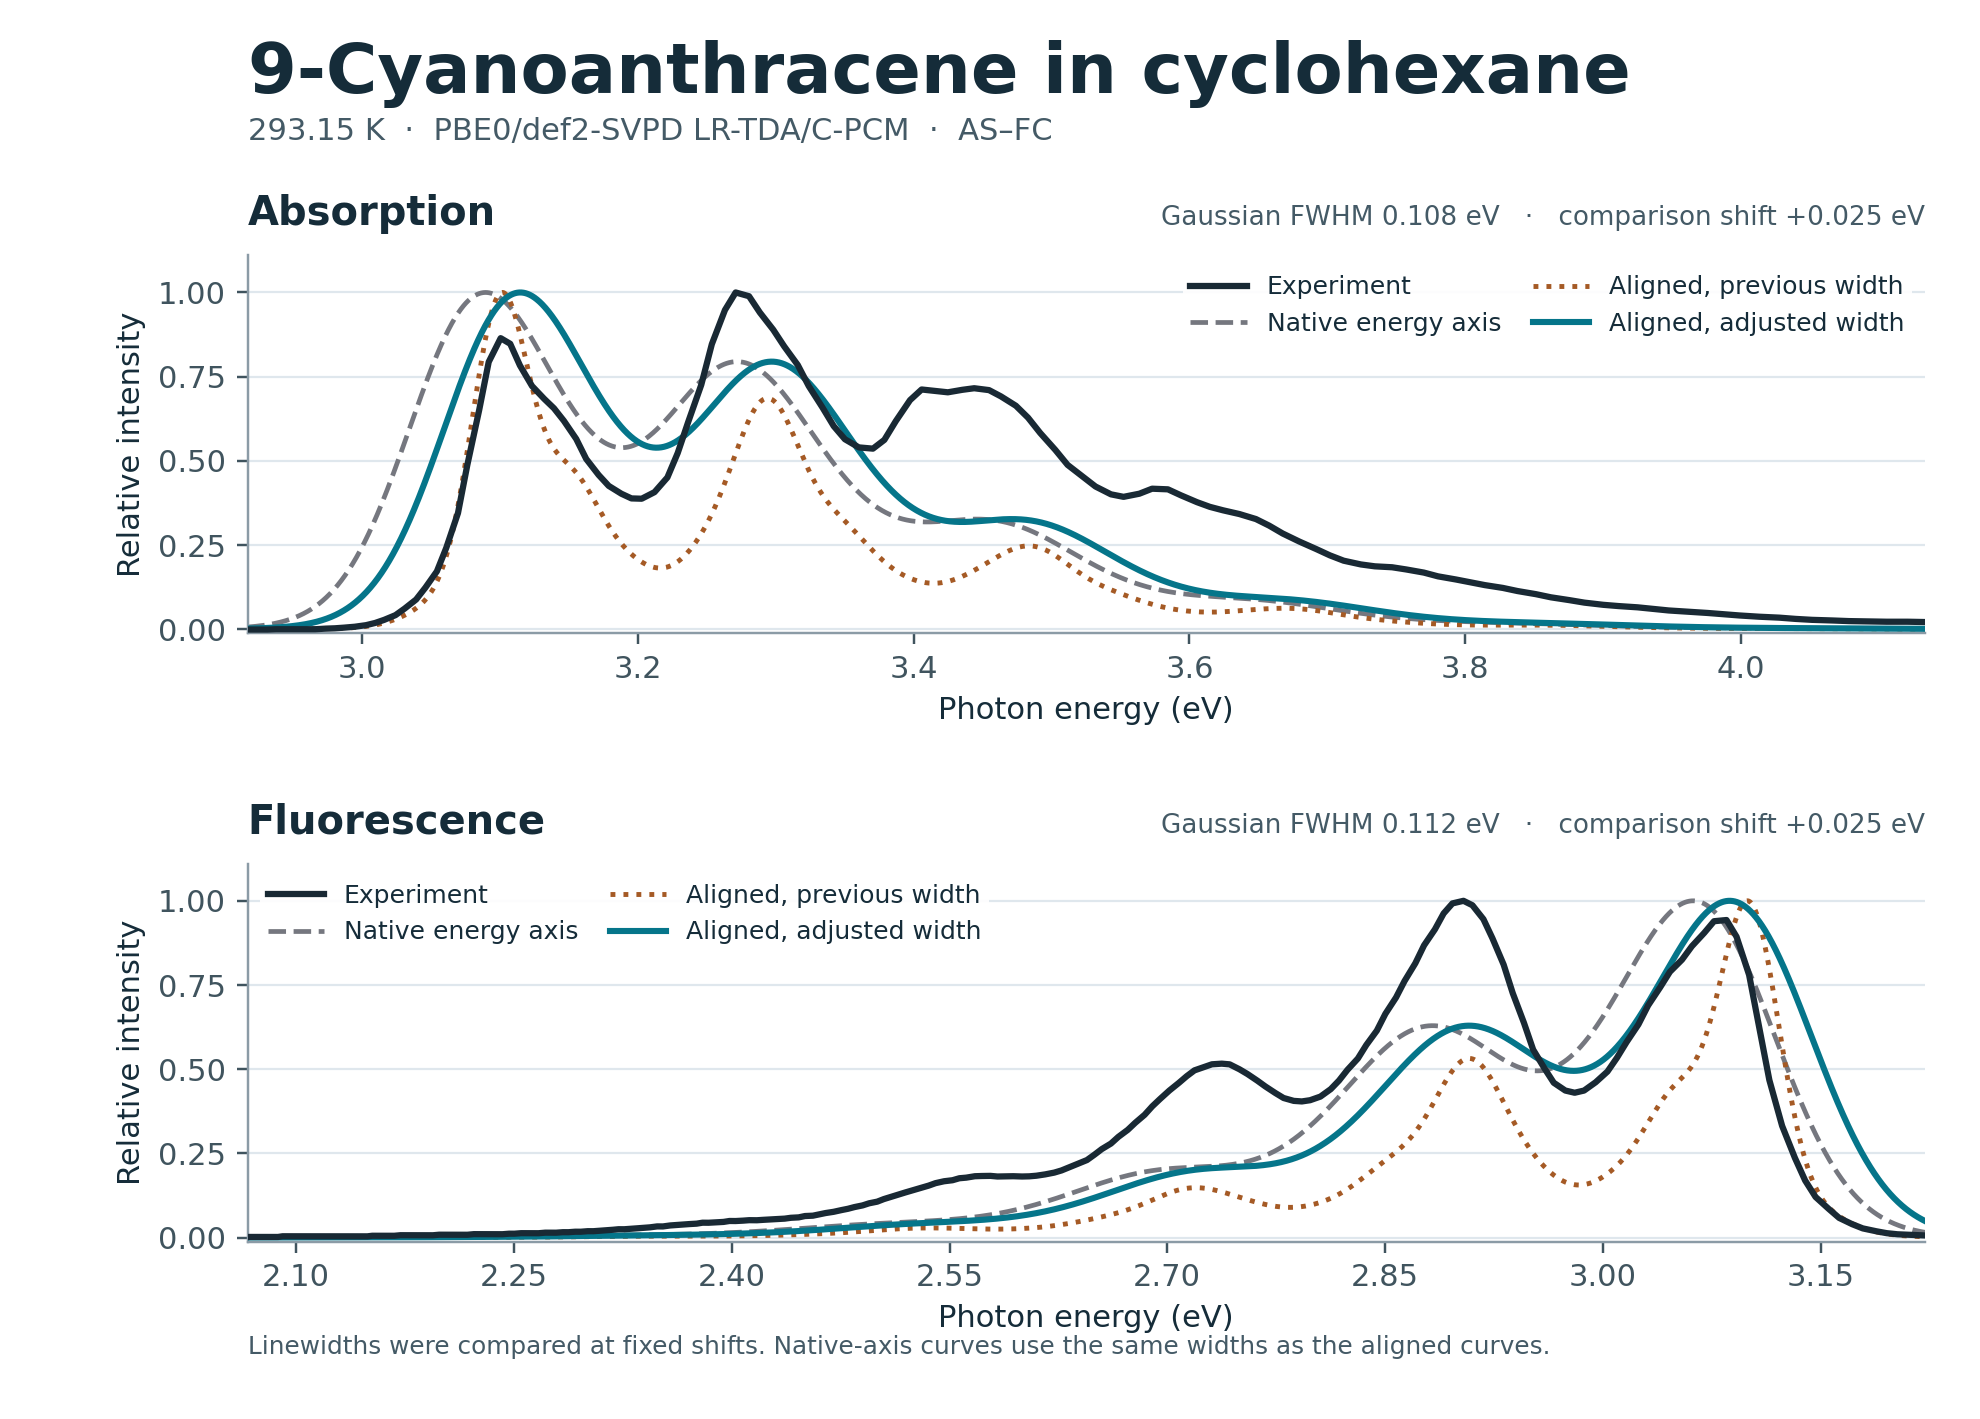
\includegraphics[width=0.88\linewidth]{cyanoanthracene.png}
  \caption{Absorption and fluorescence of 9-cyanoanthracene in cyclohexane. The equal-curvature FC calculation at 293.15 K is compared with the digitized and replotted experimental traces from Fig.~S1-D of Ref.~\cite{boens}. The fixed $+0.025$~eV shift uses the lowest-energy resolved absorption maximum at 3.10~eV as an origin proxy. The native-axis curves use the adjusted widths.}
  \label{fig:cyano}
\end{figure}

In a separate comparison on the same stationary endpoints, the analytic AH+HT model lowers the calculated origin from 24\,806.34 to 24\,228.42~\wn\ through the zero-point correction. At 80~\wn\ FWHM on the native axis, the second-to-first fluorescence band area ratio moves from 0.69 (AS--FC) to 1.37 (AH+HT), closer to the measured 1.21. The first and second integration windows span 384.85--415.97 and 415.97--443.96~nm, respectively. The calculated maxima move to 413.67 and 413.81~nm for absorption and fluorescence, respectively, increasing both absolute errors.

\subsection{Quinine dication in aqueous acid}

One diprotonated conformer, initiated from the quinine dihydrochloride hemihydrate crystal structure,\cite{quininecrystal} was modeled at density-fitted PBE0/def2-SVP/TDA\cite{weigendbasis} with a water C-PCM continuum. The 298.15 K AS--FC model uses the analytic $S_0$ Hessian for both surfaces. The absorption dipole is from optical linear response at the ground-state endpoint and the fluorescence dipole from equilibrium linear response at the relaxed excited-state endpoint. State-specific excited-state polarization and conformer populations were outside the model. The 23rd accepted excited-state step had a maximum Cartesian force component of $6.22\times10^{-5}\,E_h\,\mathrm{bohr}^{-1}$. Strict geometry convergence remained incomplete. Using the preceding accepted step changed the absorption and emission profiles by less than 0.04\% in relative integrated absolute difference.

\begin{figure}[!htbp]
  \centering
  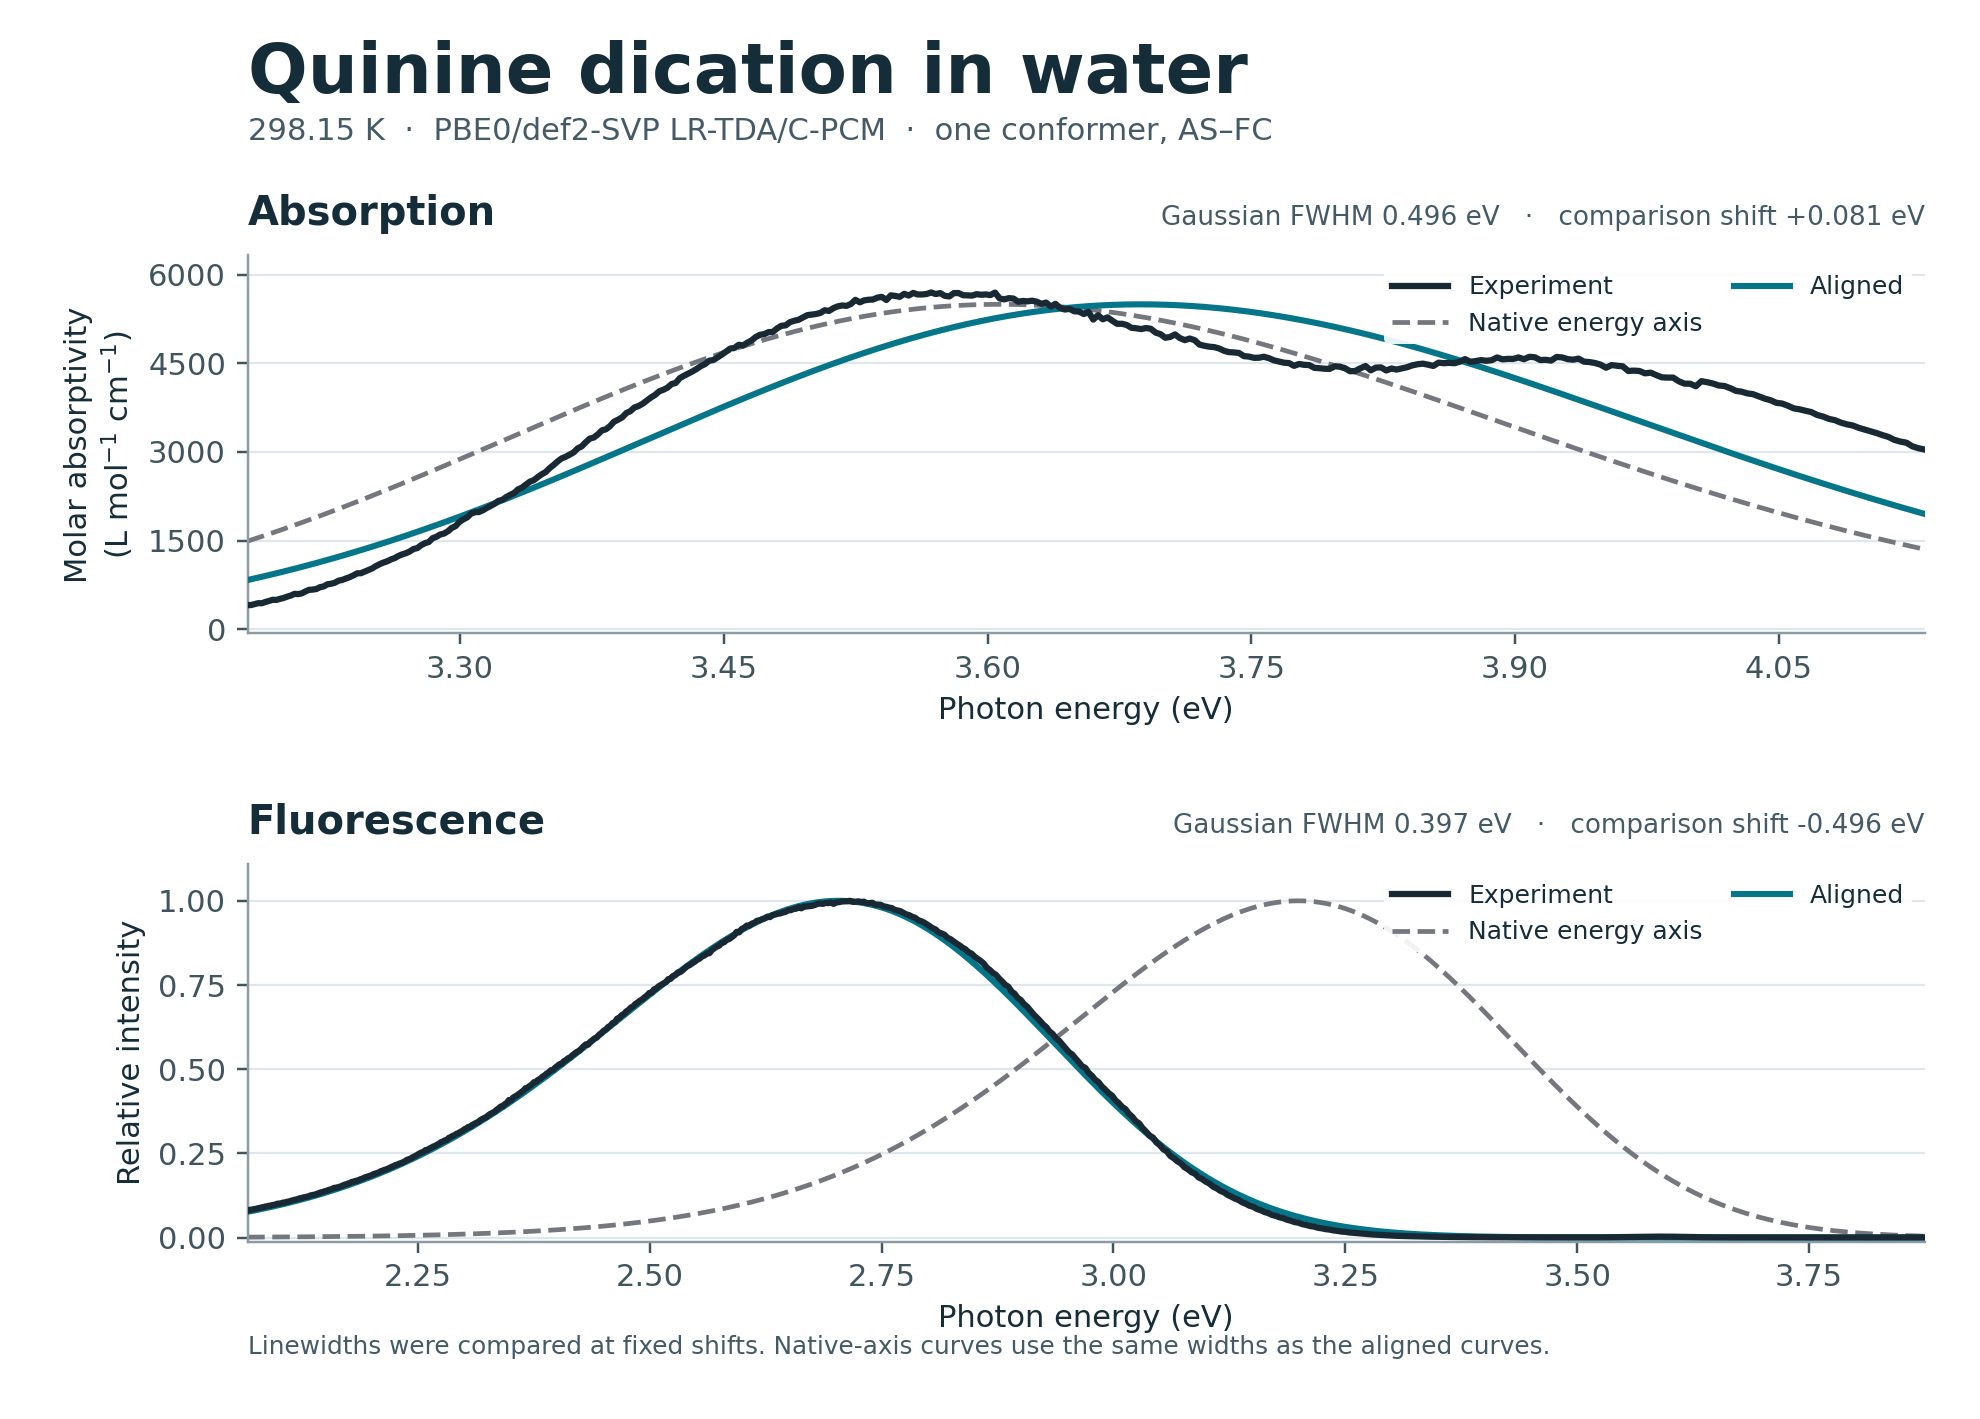
\includegraphics[width=0.86\linewidth]{quinine.png}
  \caption{Absorption and fluorescence of the quinine dication. The AS--FC calculation for one conformer in a water continuum is compared with PhotochemCAD spectra of quinine sulfate in aqueous 0.5~M sulfuric acid.\cite{photochemcad} The retained Gaussian FWHM values are 0.496~eV (absorption) and 0.397~eV (fluorescence). The translations are $+0.081$ and $-0.496$~eV, respectively. The same widths are used on the native energy axis. The absorption scale comes from the calculated oscillator strengths.}
  \label{fig:quinine}
\end{figure}

On the energy-domain plot, the measured peaks lie at 3.568 and 2.716~eV in aqueous 0.5~M sulfuric acid.\cite{photochemcad} With the broadened curves on the native axis, the calculated peaks lie at 3.606 and 3.199~eV (Fig.~\ref{fig:quinine}). Their separation is 0.407~eV, compared with 0.852~eV in the measured spectra. Independent translations move the calculated fluorescence maximum to 2.703~eV and give an RMSE of 0.0095 on the normalized energy-domain profile. The translated absorption curve gives a smaller error over the full comparison window and places the maximum at 3.687~eV. A single common shift gave a poorer joint comparison.

\subsection{Periodic-rotor diagnostic for trifluoronitrosomethane}

For the weak visible $n\pi^*$ band of CF$_3$NO,\cite{hage} a 298~K comparison used PBE0/def2-TZVPD/TDA torsional cuts with a constant effective inertia on each surface, eleven harmonic spectators, and a signed torsion-dependent transition dipole. The electronic endpoints failed the restricted-to-unrestricted orbital-stability check. The resulting reduced-model spectrum is a diagnostic of the nuclear calculation. At 80~\wn\ FWHM and on the native axis, the origin and absorption maximum are 13\,170.36 and 13\,668.86~\wn, respectively. The jet-cooled origin is 13\,929.70~\wn\ and the digitized room-temperature maximum is 14\,429.60~\wn.\cite{dyet,mason,hage} The calculated and experimental peak-to-origin intervals are 498.50 and 499.90~\wn, while the calculated maximum lies 760.74~\wn\ below the measured maximum. The small interval error in this case accompanies a nearly uniform offset of the two energy observables.

\section{Conclusions}

The examples probe distinct aspects of a vibronic calculation. Anharmonic soft-mode treatments improve the PBE benzene spectra, with residual errors in the fluorescence maxima and relative intensities. In pyridine a small relative origin error accompanies substantial errors in the strengths and locations of the bands. In 9-cyanoanthracene the analytic AH+HT model improves the relative fluorescence band areas while worsening the absolute peak positions. In quinine the equal-curvature model underestimates the absorption--fluorescence separation even though a shifted fluorescence envelope fits the measured shape. The comparisons motivate reporting the calculated energy scale, the assumptions of the electronic and vibrational models, and any empirical display parameters with each spectrum.

\section*{Code and data availability}

The \href{https://github.com/HenriqueCSJ/PySCF_ESD}{PySCF ESD repository} distributes the package under GPL-3.0-only and includes tests, benchmark drivers, and the plotted comparisons. Replaying the reported molecular calculations requires the retained electronic checkpoints and numerical spectral inputs. The experimental references identify each measured trace and the terms of reuse where specified.

\begingroup
\small
\begin{thebibliography}{99}

\bibitem{desouza} B. de Souza, F. Neese, and R. Izs\'ak, J. Chem. Phys. \textbf{148}, 034104 (2018). \doi{10.1063/1.5010895}.
\bibitem{pyscf} Q. Sun \emph{et al.}, J. Chem. Phys. \textbf{153}, 024109 (2020). \doi{10.1063/5.0006074}.
\bibitem{tda} S. Hirata and M. Head-Gordon, Chem. Phys. Lett. \textbf{314}, 291--299 (1999). \doi{10.1016/S0009-2614(99)01149-5}.
\bibitem{pbe0} C. Adamo and V. Barone, J. Chem. Phys. \textbf{110}, 6158--6170 (1999). \doi{10.1063/1.478522}.
\bibitem{diffuse} D. Rappoport and F. Furche, J. Chem. Phys. \textbf{133}, 134105 (2010). \doi{10.1063/1.3484283}.
\bibitem{stability} R. Seeger and J. A. Pople, J. Chem. Phys. \textbf{66}, 3045--3050 (1977). \doi{10.1063/1.434318}.
\bibitem{gpu} R. Li, Q. Sun, X. Zhang, and G. K.-L. Chan, J. Phys. Chem. A \textbf{129}, 1459--1468 (2025). \doi{10.1021/acs.jpca.4c05876}.
\bibitem{cpcm} M. Cossi, N. Rega, G. Scalmani, and V. Barone, J. Comput. Chem. \textbf{24}, 669--681 (2003). \doi{10.1002/jcc.10189}.
\bibitem{santoro} F. Santoro, R. Improta, A. Lami, J. Bloino, and V. Barone, J. Chem. Phys. \textbf{126}, 084509 (2007). \doi{10.1063/1.2437197}.
\bibitem{baiardi} A. Baiardi, J. Bloino, and V. Barone, J. Chem. Theory Comput. \textbf{9}, 4097--4115 (2013). \doi{10.1021/ct400450k}.
\bibitem{dvr} J. C. Light, I. P. Hamilton, and J. V. Lill, J. Chem. Phys. \textbf{82}, 1400--1409 (1985). \doi{10.1063/1.448462}.
\bibitem{laane} P. Boopalachandran and J. Laane, Chem. Phys. Lett. \textbf{462}, 178--182 (2008). \doi{10.1016/j.cplett.2008.07.080}.
\bibitem{bolovinos} A. Bolovinos, P. Tsekeris, J. Philis, E. Pantos, and G. Andritsopoulos, J. Mol. Spectrosc. \textbf{103}, 240--256 (1984). \doi{10.1016/0022-2852(84)90051-1}.
\bibitem{yamazaki} I. Yamazaki and H. Baba, J. Chem. Phys. \textbf{66}, 5826--5827 (1977). \doi{10.1063/1.433862}.
\bibitem{wang} Y. Wang, J. Ren, W. Li, and Z. Shuai, J. Phys. Chem. Lett. \textbf{13}, 6391--6399 (2022). \doi{10.1021/acs.jpclett.2c01475}.
\bibitem{boens} N. Boens \emph{et al.}, Anal. Chem. \textbf{79}, 2137--2149 (2007). \doi{10.1021/ac062160k}. \href{https://doi.org/10.1021/ac062160k.s001}{Supporting Information} (CC BY-NC 4.0).
\bibitem{quininecrystal} G. I. Anderson, S. Bellia, M. Zeller, P. C. Hillesheim, and A. Mirjafari, IUCrData \textbf{6}, x210406 (2021). \doi{10.1107/S2414314621004065}.
\bibitem{weigendbasis} F. Weigend and R. Ahlrichs, Phys. Chem. Chem. Phys. \textbf{7}, 3297--3305 (2005). \doi{10.1039/B508541A}.
\bibitem{photochemcad} R.-C. A. Fuh, quinine sulfate absorption and fluorescence, \href{https://omlc.org/spectra/PhotochemCAD/html/081.html}{PhotochemCAD entry 081}. Database described by J. M. Dixon, M. Taniguchi, and J. S. Lindsey, Photochem. Photobiol. \textbf{81}, 212--213 (2005).
\bibitem{hage} G. da S. Hage, P. H. R. de Oliveira, G. B. Ferreira, and H. C. Silva Junior, ACS Omega \textbf{11}, 64274--64282 (2026). \doi{10.1021/acsomega.6c11480}.
\bibitem{dyet} J. A. Dyet, M. R. S. McCoustra, and J. Pfab, J. Chem. Soc., Faraday Trans. 2 \textbf{84}, 463--482 (1988). \doi{10.1039/F29888400463}.
\bibitem{mason} J. Mason and J. Banus, J. Chem. Soc., 3904 (1957). \doi{10.1039/JR9570003904}.

\end{thebibliography}
\endgroup
\end{document}
